\chapter{Projekt i implementacja aplikacji}

\section{Funkcje aplikacji - diagram przypadków użycia}

\begin{figure} [H]
	\centering
	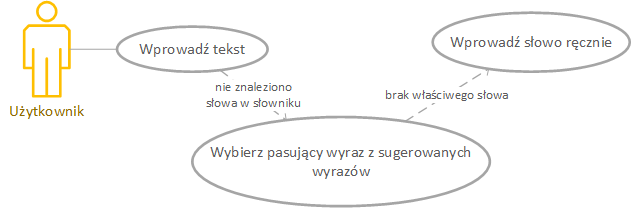
\includegraphics[width=1\linewidth]{rozdzial03/diagram.png}
	\caption{Diagram przypadków użycia}
	\label{fig:diagUzycia}
\end{figure}

Głównym zadaniem aplikacji jest wyszukiwanie błędnych wyrazów w języku polskim oraz ich korekcja. Aby tego dokonać aplikacja porównuje wyrazy znajdujące się w tekście z wyrazami znajdującymi się w słowniku. Jeśli danego słowa nie znaleziono zostaje ono uznane za błędne. Aby dokonać korekcji błędnych wyrazów stosowane są algorytmy opisane w poprzednich rozdziałach. Dla optymalizacji działania aplikacji wyszukiwanie sugestii odbywa się w osobnych wątkach co znacząco przyspiesza działanie aplikacji. 


\section{Interfejs aplikacji}

\begin{figure} [H]
	\centering
	\includegraphics[width=1\linewidth]{rozdzial03/screen1_1.png}
	\caption{Interfejs aplikacji}
	\label{fig:interfejs}
\end{figure}

\begin{enumerate}
	\item Ilość podpowiedzi - pozwala na ustawienie maksymalnej ilości podpowiedzi jakie mają się pojawić po kliknięciu prawym przyciskiem myszy na błędnie napisane słowo.
	\item Odległość Levenhteina - pozwala na ustawienie odległości jaka ma być brana pod uwagę w przypadku algorytmu Levenhstaina. Im większa liczba tym więcej podpowiedzi ale jednocześnie zmniejsza to szybkość działania aplikacji ze względu na dodatkowe obliczenia które muszą zostać wykonane. 
	\item Ilość zmian - pozwala na ustawienie parametru ilości zmian dla algorytmu podmieniającego znaki diakrytyczne. Im większa liczba tym więcej podpowiedzi oraz dłuższy czas wykonywania algorytmu.
	\item Edytor tekstu - pozwala na edycję tekstu. Wyszukiwanie błędów działa w czasie rzeczywistym (funkcja sprawdzająca poprawność uruchamia się z każdym kliknięciem spacji). Jeśli dane słowo zostało uznane za błędne zostaje zaznaczone kolorem czerwonym. Aby je poprawić należy kliknąć na nie prawym przyciskiem myszki. Zostanie wyświetlone menu kontekstowe zawierające możliwe zamienniki. Aby podmienić słowo wystarczy kliknąć na zamiennik. Możliwe jest również poprawienie tekstu ręcznie wpisując w miejscu błędnego słowa poprawne. 
	
\end{enumerate}

\section{Wpływ parametrów na wyniki wyszukiwania}

\begin{figure} [H]
	\centering
	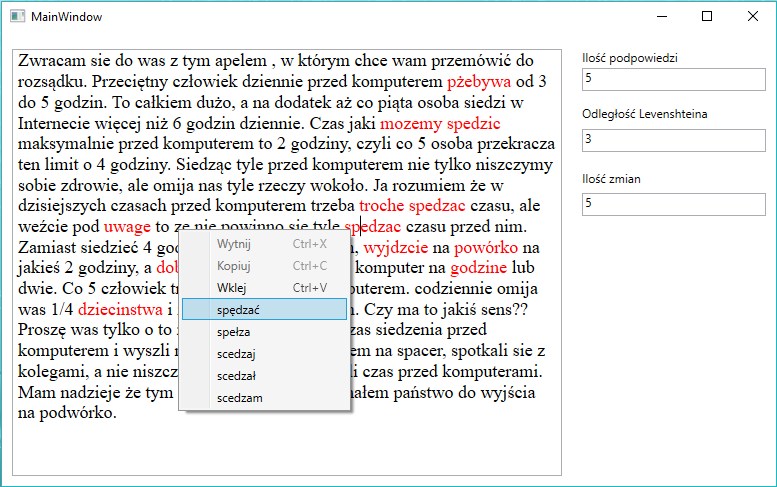
\includegraphics[width=1\linewidth]{rozdzial03/screen2.png}
	\caption{Przykładowy wynik wyszukiwania sugestii}
	\label{fig:interfejs1}
\end{figure}

\begin{figure} [H]
	\centering
	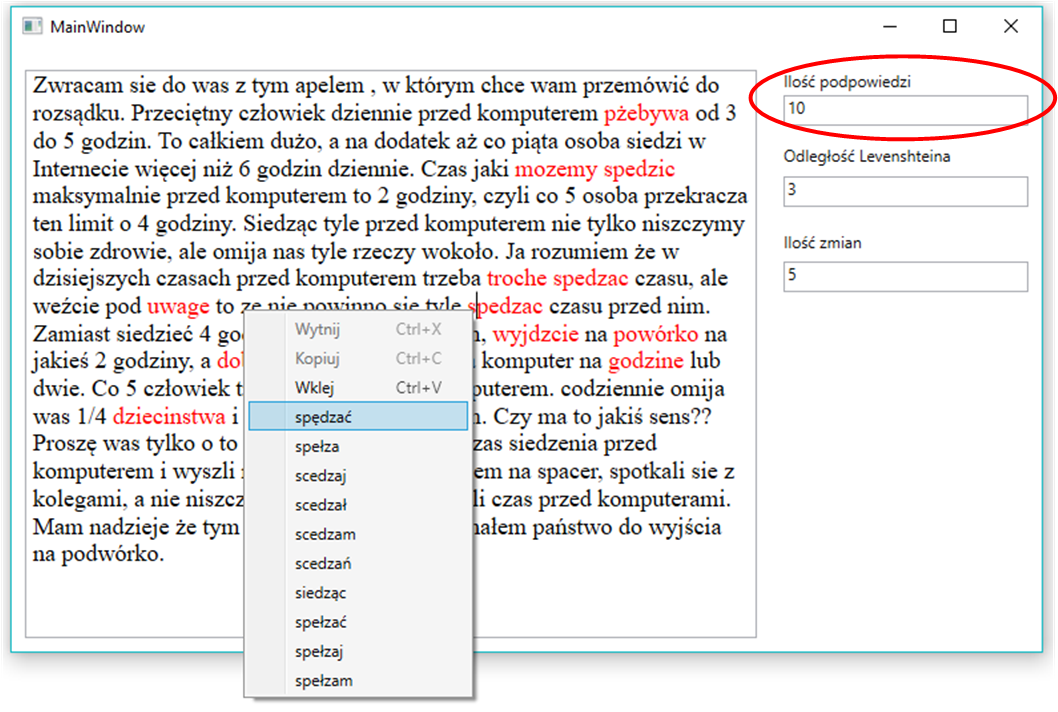
\includegraphics[width=1\linewidth]{rozdzial03/screen3_1.png}
	\caption{Zwiększenie ilości wyświetlanych sugestii}
	\label{fig:interfejs2}
\end{figure}

\begin{figure} [H]
	\centering
	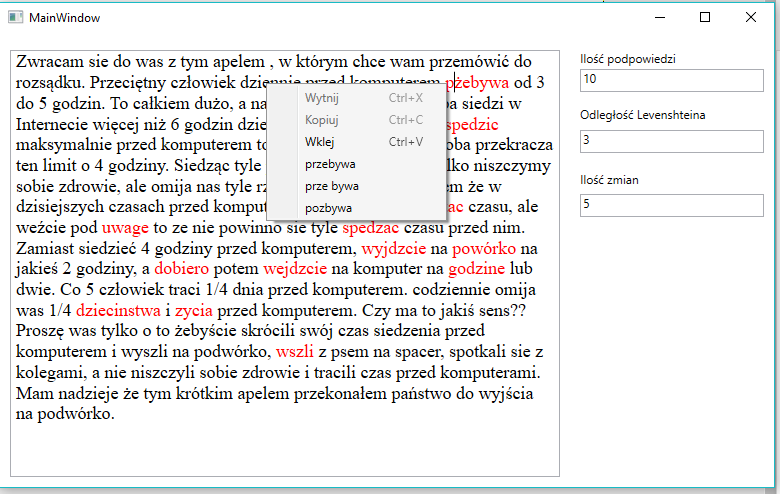
\includegraphics[width=1\linewidth]{rozdzial03/screen4.png}
	\caption{Przykładowy wynik wyszukiwania sugestii dla małej ilości podpowiedzi}
	\label{fig:interfejs3}
\end{figure}

\begin{figure} [H]
	\centering
	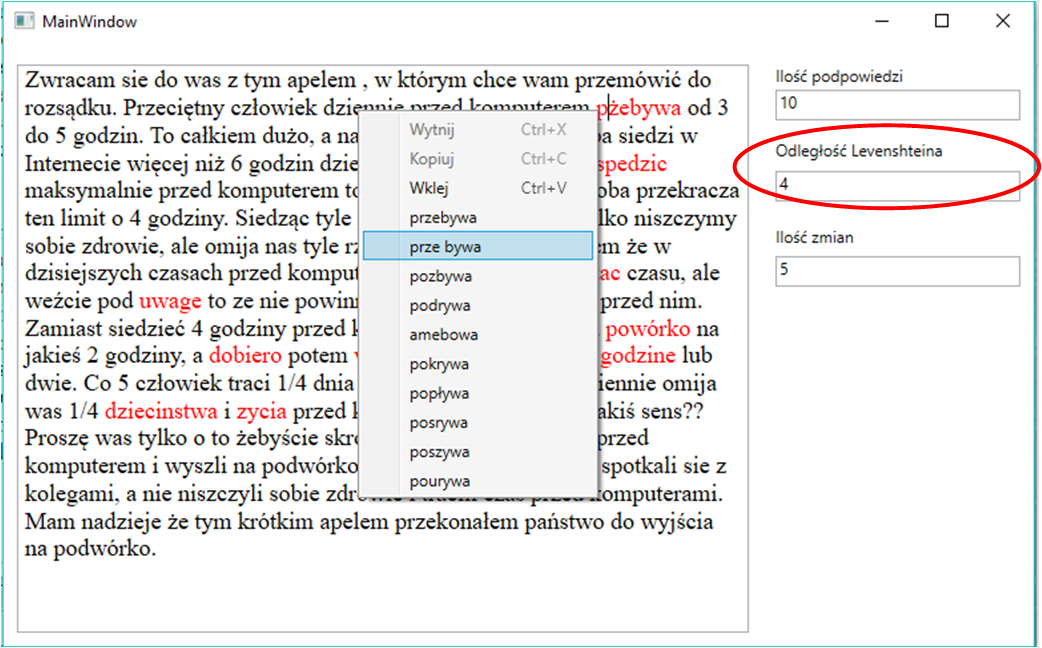
\includegraphics[width=1\linewidth]{rozdzial03/screen5_1.png}
	\caption{Zwiększenie odległości Levenhstaina}
	\label{fig:interfejs4}
\end{figure}

\begin{figure} [H]
	\centering
	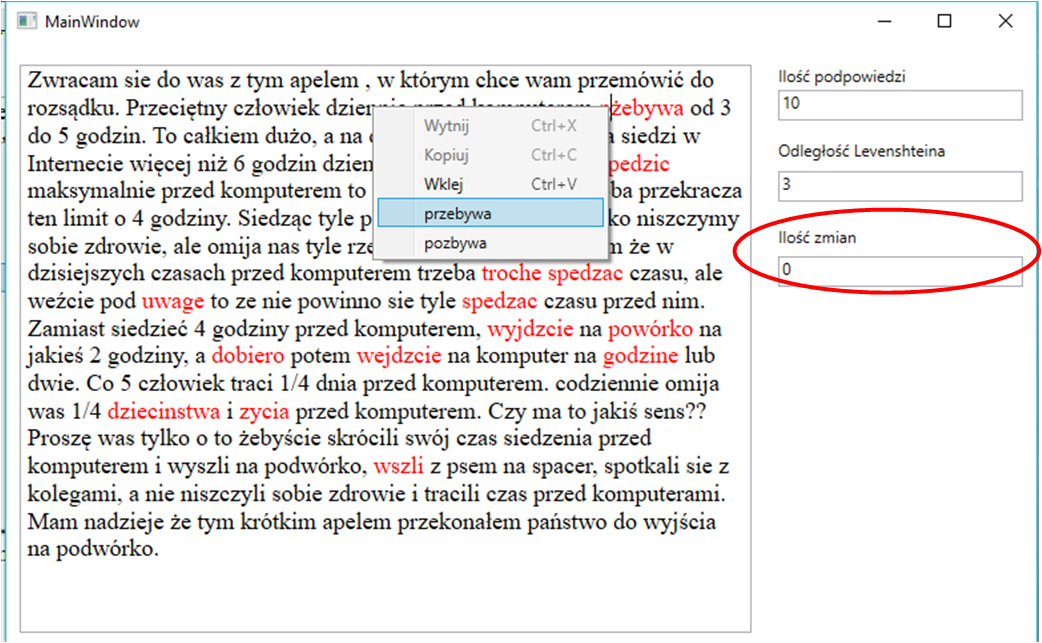
\includegraphics[width=1\linewidth]{rozdzial03/screen6_1.png}
	\caption{Zwiększenie ilości zmian}
	\label{fig:interfejs5}
\end{figure}

\section{Realizacja wybranych funkcjonalności}

\begin{figure} [H]
	\centering
	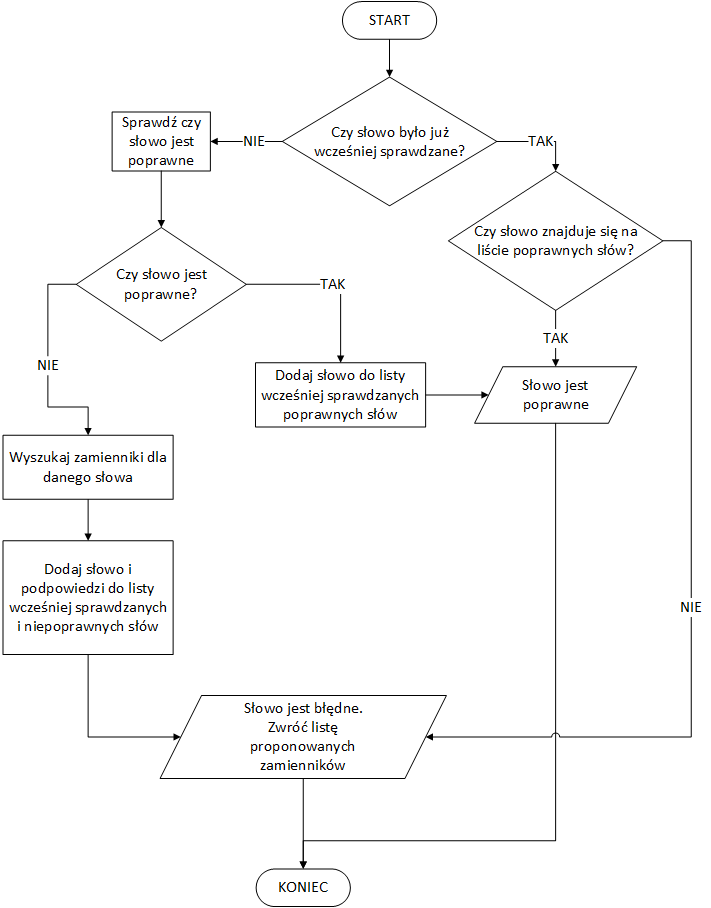
\includegraphics[width=1\linewidth]{rozdzial03/CorectorManager.png}
	\caption{Korekcja tekstu z poziomu interfejsu}
	\label{fig:CorectorManager}
\end{figure}
